\section {Two linked lists that merge (Algorithms)}

You are given two singly linked lists that merge at some element, from which point on they share the same tail:

\begin{center}
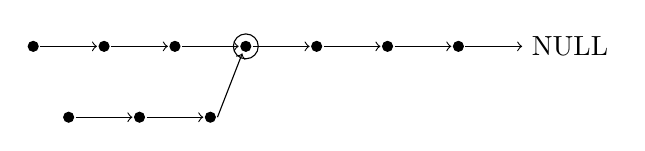
\begin{tikzpicture}[scale=.9]
\foreach \x in {0,...,6} {
	\filldraw (\x,0) circle (2pt);
}
\foreach \x in {0,...,5} {
	\draw[->] (\x+.1,0) -- (\x+.9,0);
}
\draw[->] (6.1,0) -- (6.9,0) node[right] {NULL};
\foreach \x in {1,2,3} {
	\filldraw (\x-.5,-1) circle (2pt);
}
\draw[->] (.6,-1) -- (1.4,-1);
\draw[->] (1.6,-1) -- (2.4,-1);
\draw[->] (2.6,-1) -- (2.95,-.1);
\draw (3,0) circle (5pt);
\end{tikzpicture}
\end{center}

Find the first element that is common to both lists (circled in the drawing), in linear time and using $O(1)$ memory.

\subsection{Solution}

Walk over both lists to find their lengths $l_1$ and $l_2$. The common tail has the same length in both lists,
so the longer list has exactly $|l_1 - l_2|$ extra elements before the merge, compared to the shorter one.

Put a pointer at the start of the shorter list and another pointer $|l_1 - l_2|$ elements into the longer list.
Now both pointers are the same distance from the end. Advance them together, one element at a time, until they point to the same element.
That element is the first common element.
Since both pointers are the same distance from the merge, they reach it at the same time.

This takes $O(l_1 + l_2)$ time and needs only a few variables.
